\documentclass[tikz,border=8pt]{standalone}
\usepackage{amsmath}
\usetikzlibrary{arrows.meta,calc}

\definecolor{ink}{HTML}{21352F}
\definecolor{teal}{HTML}{087F7B}
\definecolor{blue}{HTML}{4B77A8}
\definecolor{gold}{HTML}{C58B2A}
\definecolor{rose}{HTML}{B65A62}

\begin{document}
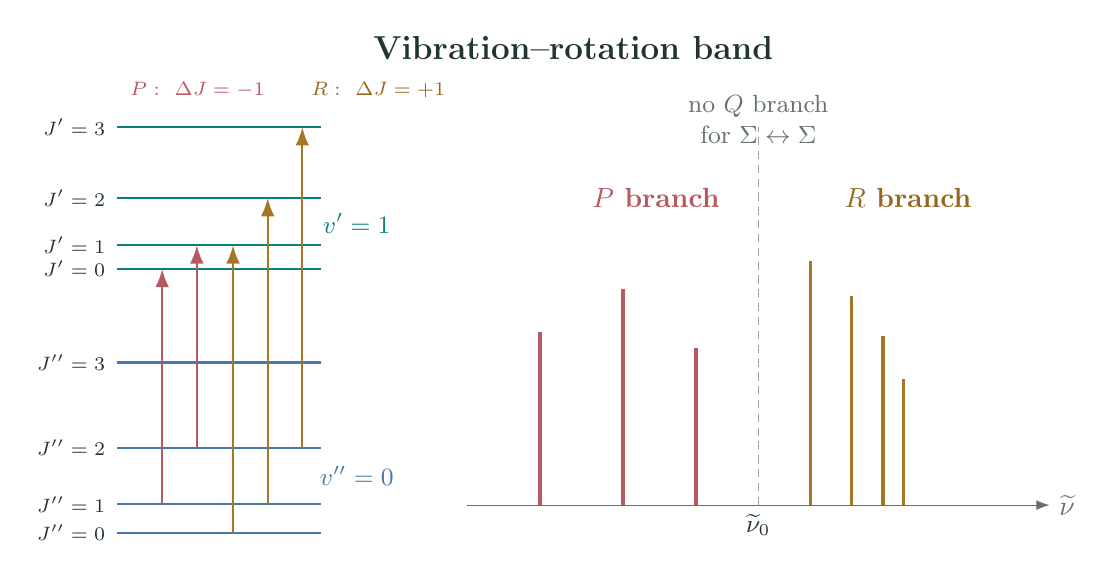
\begin{tikzpicture}[font=\sffamily,text=ink,>=Latex]
  \node[font=\bfseries\large] at (0,6.15)
    {Vibration--rotation band};

  \foreach \J in {0,...,3}{
    \pgfmathsetmacro{\yl}{0.18*\J*(\J+1)}
    \pgfmathsetmacro{\yu}{3.35+0.15*\J*(\J+1)}
    \draw[blue,thick] (-5.8,\yl)--(-3.2,\yl);
    \draw[teal,thick] (-5.8,\yu)--(-3.2,\yu);
    \node[left,font=\scriptsize] at (-5.82,\yl) {$J''=\J$};
    \node[left,font=\scriptsize] at (-5.82,\yu) {$J'=\J$};
  }
  \node[blue,font=\small] at (-2.75,.72) {$v''=0$};
  \node[teal,font=\small] at (-2.75,3.93) {$v'=1$};

  % P(1), P(2)
  \draw[rose,thick,->] (-5.22,.36)--(-5.22,3.35);
  \draw[rose,thick,->] (-4.78,1.08)--(-4.78,3.65);
  % R(0), R(1), R(2)
  \draw[gold!85!black,thick,->] (-4.32,0)--(-4.32,3.65);
  \draw[gold!85!black,thick,->] (-3.88,.36)--(-3.88,4.25);
  \draw[gold!85!black,thick,->] (-3.44,1.08)--(-3.44,5.15);
  \node[rose,font=\scriptsize\bfseries,anchor=west] at (-5.75,5.62)
    {$P:\ \Delta J=-1$};
  \node[gold!75!black,font=\scriptsize\bfseries,anchor=west] at (-3.45,5.62)
    {$R:\ \Delta J=+1$};

  \draw[->,ink!70] (-1.35,.35)--(6.05,.35)
    node[right] {$\widetilde\nu$};
  \coordinate (O) at (2.35,.35);
  \draw[ink!45,densely dashed] (O)--(2.35,5.15);
  \node[below,font=\small] at (O) {$\widetilde\nu_0$};

  % The spectral positions use the same B'=0.15 and B''=0.18
  % as the level diagram at left.
  \pgfmathsetmacro{\Bupper}{0.15}
  \pgfmathsetmacro{\Blower}{0.18}
  \pgfmathsetmacro{\xscale}{2.2}
  \pgfmathsetmacro{\xzero}{2.35}
  \foreach \J/\h in {1/2.35,2/3.10,3/2.55}{
    \pgfmathsetmacro{\shift}{
      \Bupper*(\J-1)*\J-\Blower*\J*(\J+1)}
    \pgfmathsetmacro{\xx}{\xzero+\xscale*\shift}
    \draw[rose,very thick] (\xx,.35)--(\xx,\h);
  }
  \foreach \J/\h in {0/3.45,1/3.00,2/2.50,3/1.95}{
    \pgfmathsetmacro{\shift}{
      \Bupper*(\J+1)*(\J+2)-\Blower*\J*(\J+1)}
    \pgfmathsetmacro{\xx}{\xzero+\xscale*\shift}
    \draw[gold!85!black,very thick] (\xx,.35)--(\xx,\h);
  }
  \node[rose,font=\bfseries] at (1.05,4.25) {$P$ branch};
  \node[gold!75!black,font=\bfseries] at (4.25,4.25) {$R$ branch};
  \node[font=\small,align=center,text=ink!70] at (2.35,5.25)
    {no $Q$ branch\\for $\Sigma\leftrightarrow\Sigma$};
\end{tikzpicture}
\end{document}
